% Options for packages loaded elsewhere
\PassOptionsToPackage{unicode}{hyperref}
\PassOptionsToPackage{hyphens}{url}
%
\documentclass[
]{article}
\usepackage{amsmath,amssymb}
\usepackage{lmodern}
\usepackage{iftex}
\ifPDFTeX
  \usepackage[T1]{fontenc}
  \usepackage[utf8]{inputenc}
  \usepackage{textcomp} % provide euro and other symbols
\else % if luatex or xetex
  \usepackage{unicode-math}
  \defaultfontfeatures{Scale=MatchLowercase}
  \defaultfontfeatures[\rmfamily]{Ligatures=TeX,Scale=1}
\fi
% Use upquote if available, for straight quotes in verbatim environments
\IfFileExists{upquote.sty}{\usepackage{upquote}}{}
\IfFileExists{microtype.sty}{% use microtype if available
  \usepackage[]{microtype}
  \UseMicrotypeSet[protrusion]{basicmath} % disable protrusion for tt fonts
}{}
\makeatletter
\@ifundefined{KOMAClassName}{% if non-KOMA class
  \IfFileExists{parskip.sty}{%
    \usepackage{parskip}
  }{% else
    \setlength{\parindent}{0pt}
    \setlength{\parskip}{6pt plus 2pt minus 1pt}}
}{% if KOMA class
  \KOMAoptions{parskip=half}}
\makeatother
\usepackage{xcolor}
\usepackage[left=3cm,right=3cm,top=2cm,bottom=2cm]{geometry}
\usepackage{longtable,booktabs,array}
\usepackage{calc} % for calculating minipage widths
% Correct order of tables after \paragraph or \subparagraph
\usepackage{etoolbox}
\makeatletter
\patchcmd\longtable{\par}{\if@noskipsec\mbox{}\fi\par}{}{}
\makeatother
% Allow footnotes in longtable head/foot
\IfFileExists{footnotehyper.sty}{\usepackage{footnotehyper}}{\usepackage{footnote}}
\makesavenoteenv{longtable}
\usepackage{graphicx}
\makeatletter
\def\maxwidth{\ifdim\Gin@nat@width>\linewidth\linewidth\else\Gin@nat@width\fi}
\def\maxheight{\ifdim\Gin@nat@height>\textheight\textheight\else\Gin@nat@height\fi}
\makeatother
% Scale images if necessary, so that they will not overflow the page
% margins by default, and it is still possible to overwrite the defaults
% using explicit options in \includegraphics[width, height, ...]{}
\setkeys{Gin}{width=\maxwidth,height=\maxheight,keepaspectratio}
% Set default figure placement to htbp
\makeatletter
\def\fps@figure{htbp}
\makeatother
\setlength{\emergencystretch}{3em} % prevent overfull lines
\providecommand{\tightlist}{%
  \setlength{\itemsep}{0pt}\setlength{\parskip}{0pt}}
\setcounter{secnumdepth}{5}
% ---
% Pacotes básicos 
% ---
\usepackage{lmodern}			% Usa a fonte Latin Modern			
\usepackage[T1]{fontenc}		% Selecao de codigos de fonte.
\usepackage[utf8]{inputenc}		% Codificacao do documento (conversão automática dos acentos)
\usepackage{indentfirst}		% Indenta o primeiro parágrafo de cada seção.
\usepackage{color}				% Controle das cores
\usepackage{graphicx}			% Inclusão de gráficos
\usepackage{microtype} 			% para melhorias de justificação
% ---

\usepackage{tocloft}

\cftsetindents{section}{0em}{2em}
\cftsetindents{subsection}{0em}{2em}

\renewcommand\cfttoctitlefont{\hfill\LARGE\bfseries}
\renewcommand\cftaftertoctitle{\hfill\mbox{}}

\setcounter{tocdepth}{3}

\usepackage[portuguese]{babel}


\renewcommand{\contentsname}{Sumário}
\usepackage{booktabs}
\usepackage{longtable}
\usepackage{array}
\usepackage{multirow}
\usepackage{wrapfig}
\usepackage{float}
\usepackage{colortbl}
\usepackage{pdflscape}
\usepackage{tabu}
\usepackage{threeparttable}
\usepackage{threeparttablex}
\usepackage[normalem]{ulem}
\usepackage{makecell}
\usepackage{xcolor}
\ifLuaTeX
  \usepackage{selnolig}  % disable illegal ligatures
\fi
\IfFileExists{bookmark.sty}{\usepackage{bookmark}}{\usepackage{hyperref}}
\IfFileExists{xurl.sty}{\usepackage{xurl}}{} % add URL line breaks if available
\urlstyle{same} % disable monospaced font for URLs
\hypersetup{
  pdftitle={Soluções de problemas do livro Econometria Básica (Gujarati, Porter)},
  pdfauthor={Igo da Costa Andrade},
  hidelinks,
  pdfcreator={LaTeX via pandoc}}

\title{Soluções de problemas do livro \emph{Econometria Básica (Gujarati, Porter)}}
\author{Igo da Costa Andrade}
\date{2023-06-01}

\begin{document}
\maketitle

{
\setcounter{tocdepth}{2}
\tableofcontents
}
\newpage

\hypertarget{informauxe7uxf5es-preliminares}{%
\section*{Informações preliminares}\label{informauxe7uxf5es-preliminares}}
\addcontentsline{toc}{section}{Informações preliminares}

GUJARATI, Damodar N.; PORTER, Dawn C. \textbf{Econometria básica}. 5. ed.~São Paulo: Amgh Editora, 2011.

\begin{center}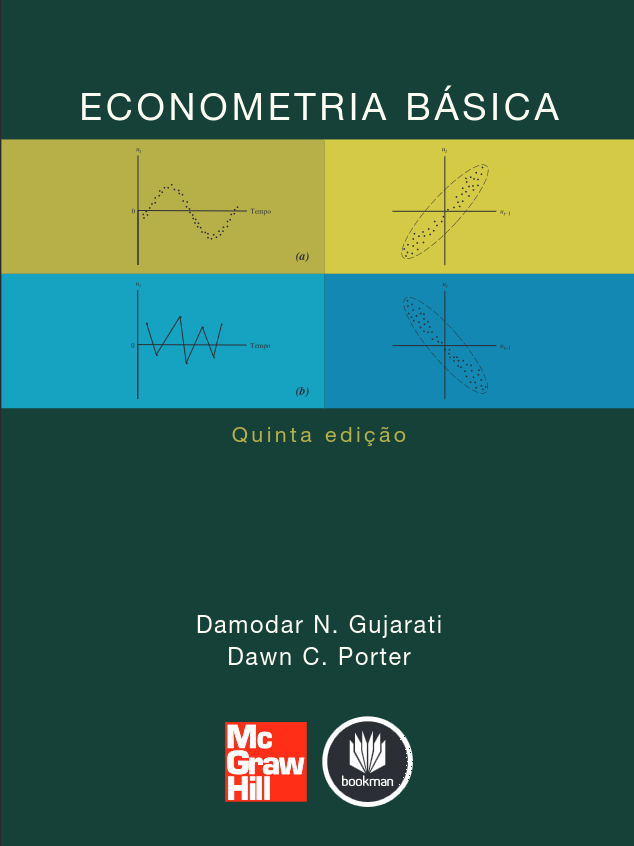
\includegraphics[width=0.5\linewidth]{assets/images/econometria_gujarati_capa} \end{center}

\newpage

\hypertarget{a-natureza-da-anuxe1lise-de-regressuxe3o}{%
\section{A natureza da análise de regressão}\label{a-natureza-da-anuxe1lise-de-regressuxe3o}}

\hypertarget{exercuxedcios}{%
\subsection*{Exercícios}\label{exercuxedcios}}

\begin{enumerate}
\def\labelenumi{\arabic{enumi}.}
\item
  A Tabela 1.3 apresenta dados relativos ao Índice de Preços ao Consumidor (IPC) de sete países
  industrializados. A base do índice é 1982--1984 = 100.

  \begin{table}[H]

   \caption{\label{tab:unnamed-chunk-3}IPC em sete países industrializados, 1980-2005 (1982-1984=100) [Tab. 1.3]}
   \centering
   \begin{tabular}[t]{rrrrrrrr}
   \toprule
   Ano & EUA & Canadá & Japão & França & Alemanha & Itália & Reino Unido\\
   \midrule
   \cellcolor{gray!6}{1980} & \cellcolor{gray!6}{82.4} & \cellcolor{gray!6}{76.1} & \cellcolor{gray!6}{90.9} & \cellcolor{gray!6}{72.3} & \cellcolor{gray!6}{86.7} & \cellcolor{gray!6}{63.2} & \cellcolor{gray!6}{78.5}\\
   1981 & 90.9 & 85.6 & 95.3 & 81.9 & 92.2 & 75.4 & 87.9\\
   \cellcolor{gray!6}{1982} & \cellcolor{gray!6}{96.5} & \cellcolor{gray!6}{94.9} & \cellcolor{gray!6}{98.1} & \cellcolor{gray!6}{91.7} & \cellcolor{gray!6}{97.1} & \cellcolor{gray!6}{87.7} & \cellcolor{gray!6}{95.4}\\
   1983 & 99.6 & 100.4 & 99.8 & 100.4 & 100.3 & 100.8 & 99.8\\
   \cellcolor{gray!6}{1984} & \cellcolor{gray!6}{103.9} & \cellcolor{gray!6}{104.7} & \cellcolor{gray!6}{102.1} & \cellcolor{gray!6}{108.1} & \cellcolor{gray!6}{102.7} & \cellcolor{gray!6}{111.5} & \cellcolor{gray!6}{104.8}\\
   1985 & 107.6 & 109.0 & 104.2 & 114.4 & 104.8 & 121.1 & 111.1\\
   \cellcolor{gray!6}{1986} & \cellcolor{gray!6}{109.6} & \cellcolor{gray!6}{113.5} & \cellcolor{gray!6}{104.9} & \cellcolor{gray!6}{117.3} & \cellcolor{gray!6}{104.7} & \cellcolor{gray!6}{128.5} & \cellcolor{gray!6}{114.9}\\
   1987 & 113.6 & 118.4 & 104.9 & 121.1 & 104.9 & 134.4 & 119.7\\
   \cellcolor{gray!6}{1988} & \cellcolor{gray!6}{118.3} & \cellcolor{gray!6}{123.2} & \cellcolor{gray!6}{105.6} & \cellcolor{gray!6}{124.4} & \cellcolor{gray!6}{106.3} & \cellcolor{gray!6}{141.1} & \cellcolor{gray!6}{125.6}\\
   1989 & 124.0 & 129.3 & 108.0 & 128.7 & 109.2 & 150.4 & 135.3\\
   \cellcolor{gray!6}{1990} & \cellcolor{gray!6}{130.7} & \cellcolor{gray!6}{135.5} & \cellcolor{gray!6}{111.4} & \cellcolor{gray!6}{133.0} & \cellcolor{gray!6}{112.2} & \cellcolor{gray!6}{159.6} & \cellcolor{gray!6}{148.2}\\
   1991 & 136.2 & 143.1 & 115.0 & 137.2 & 116.3 & 169.8 & 156.9\\
   \cellcolor{gray!6}{1992} & \cellcolor{gray!6}{140.3} & \cellcolor{gray!6}{145.3} & \cellcolor{gray!6}{117.0} & \cellcolor{gray!6}{140.5} & \cellcolor{gray!6}{122.1} & \cellcolor{gray!6}{178.8} & \cellcolor{gray!6}{162.7}\\
   1993 & 144.5 & 147.9 & 118.5 & 143.5 & 127.6 & 186.4 & 165.3\\
   \cellcolor{gray!6}{1994} & \cellcolor{gray!6}{148.2} & \cellcolor{gray!6}{148.2} & \cellcolor{gray!6}{119.3} & \cellcolor{gray!6}{145.8} & \cellcolor{gray!6}{131.1} & \cellcolor{gray!6}{193.7} & \cellcolor{gray!6}{169.4}\\
   1995 & 152.4 & 151.4 & 119.2 & 148.4 & 133.5 & 204.1 & 175.1\\
   \cellcolor{gray!6}{1996} & \cellcolor{gray!6}{156.9} & \cellcolor{gray!6}{153.8} & \cellcolor{gray!6}{119.3} & \cellcolor{gray!6}{151.4} & \cellcolor{gray!6}{135.5} & \cellcolor{gray!6}{212.0} & \cellcolor{gray!6}{179.4}\\
   1997 & 160.5 & 156.3 & 121.5 & 153.2 & 137.8 & 215.7 & 185.0\\
   \cellcolor{gray!6}{1998} & \cellcolor{gray!6}{163.0} & \cellcolor{gray!6}{157.8} & \cellcolor{gray!6}{122.2} & \cellcolor{gray!6}{154.2} & \cellcolor{gray!6}{139.1} & \cellcolor{gray!6}{222.5} & \cellcolor{gray!6}{191.4}\\
   1999 & 166.6 & 160.5 & 121.8 & 155.0 & 140.0 & 226.2 & 194.3\\
   \cellcolor{gray!6}{2000} & \cellcolor{gray!6}{172.2} & \cellcolor{gray!6}{164.9} & \cellcolor{gray!6}{121.0} & \cellcolor{gray!6}{157.6} & \cellcolor{gray!6}{142.0} & \cellcolor{gray!6}{231.9} & \cellcolor{gray!6}{200.1}\\
   2001 & 177.1 & 169.1 & 120.1 & 160.2 & 144.8 & 238.3 & 203.6\\
   \cellcolor{gray!6}{2002} & \cellcolor{gray!6}{179.9} & \cellcolor{gray!6}{172.9} & \cellcolor{gray!6}{119.0} & \cellcolor{gray!6}{163.3} & \cellcolor{gray!6}{146.7} & \cellcolor{gray!6}{244.3} & \cellcolor{gray!6}{207.0}\\
   2003 & 184.0 & 177.7 & 118.7 & 166.7 & 148.3 & 250.8 & 213.0\\
   \cellcolor{gray!6}{2004} & \cellcolor{gray!6}{188.9} & \cellcolor{gray!6}{181.0} & \cellcolor{gray!6}{118.7} & \cellcolor{gray!6}{170.3} & \cellcolor{gray!6}{150.8} & \cellcolor{gray!6}{256.3} & \cellcolor{gray!6}{219.4}\\
   2005 & 195.3 & 184.9 & 118.3 & 173.2 & 153.7 & 261.3 & 225.6\\
   \bottomrule
   \end{tabular}
   \end{table}

  \begin{enumerate}
  \def\labelenumii{\alph{enumii}.}
  \tightlist
  \item
    Com base nos dados fornecidos, calcule a taxa de inflação de cada país.
  \item
    Represente graficamente a taxa de inflação de cada país em relação ao tempo (isto é, use o eixo horizontal para o tempo e o eixo vertical para a taxa de inflação).
  \item
    Que conclusões gerais é possível tirar sobre a evolução da inflação nos sete países?
  \item
    Em que país a taxa de inflação parece ser a mais flutuante? Há alguma explicação para isso?
  \end{enumerate}
\end{enumerate}

\newpage

\hypertarget{anuxe1lise-de-regressuxe3o-com-duas-variuxe1veis-algumas-ideias-buxe1sicas}{%
\section{Análise de regressão com duas variáveis: algumas ideias básicas}\label{anuxe1lise-de-regressuxe3o-com-duas-variuxe1veis-algumas-ideias-buxe1sicas}}

\newpage

\hypertarget{modelo-de-regressuxe3o-de-duas-variuxe1veis-o-problema-da-estimauxe7uxe3o}{%
\section{Modelo de regressão de duas variáveis: o problema da estimação}\label{modelo-de-regressuxe3o-de-duas-variuxe1veis-o-problema-da-estimauxe7uxe3o}}

\end{document}
